
\chapter*{Comunicação entre processos e sincronização}

Comunicação entre processos (IPC -- {\it Inter-process communication})
e sincronização são divididas em três grandes categorias:

\begin{enumerate}

\item Comunicação: relacionada à troca de dados entre os processos;
\item Sincronização: coordenação das ações dos processos ou threads;
\item Sinais: podem ser utilizados com técnica de sincronização.

\end{enumerate}

\section*{Comunicação}

\begin{itemize}
\item Transferência de dados: relacionada à leitura e escrita em
  arquivos. Por exemplo, um processo escreve enquanto outro lê a
  escrita deste processo;

\item Memória compartilhada: uma região de memória contendo
  informações é compartilhada entre os processos.
  
\end{itemize}

\subsection*{Transferência de dados}

\begin{itemize}

\item Fluxo de dados: dados transferidos via {\it pipe}, FIFO ou {\it
  socket}, onde cada operação lê um número arbitrário de bytes,
  independente do tamanho dos blocos escritos. Como exemplo, temos a
  concatenação de comandos shell, como o descrito a seguir, onde a
  saída do comando {\tt ls} é escrita na entrada do comando {\tt wc}:

\noindent{\tt \$ ls $|$ wc \hfill\scriptsize\# pipe de comandos shell} 

\begin{center}
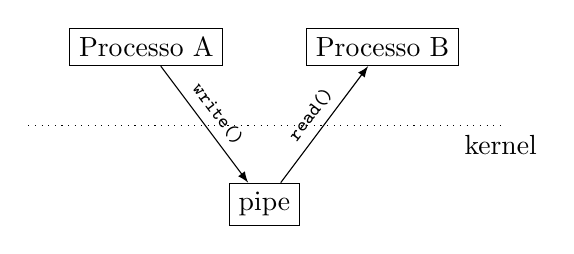
\begin{tikzpicture}
\def\shift{3cm}
\def\yshift{\shift/3}
\tikzset{base/.style={draw},pipe/.style={base},proc/.style={base},
every path/.style={>=latex,draw},syscal/.style={font=\scriptsize\tt}}
\node[pipe] at (\shift,-\yshift) (PIPE) {pipe};
\draw[dotted] (0,0) -- (2*\shift,0) node[below] {kernel};
\node[proc] at (\shift/2,\yshift) (PA) {Processo A};
\node[proc] at (1.5*\shift,\yshift) (PB) {Processo B};
\path[->] (PA) -- node[syscal,rotate=-53,above]{write()} (PIPE);
\path[->] (PIPE) -- node[syscal,rotate=53,above]{read()} (PB);
\end{tikzpicture}
\end{center}


\item Mensagem: os dados são trocados criando uma fila contendo-os
  em partes de tamanho fixo chamadas mensagens. O processo lê uma
  mensagem por vez na fila, é não é possível ler somente parte da
  mensagem.

\begin{center}
\begin{tikzpicture}
\def\shift{3cm}
\def\yshift{\shift/1.5}
\tikzset{
base/.style={draw,font=\small},
queue/.style={base,minimum width=2*\shift,minimum height=\shift/6,align=center},
proc/.style={base},
every path/.style={>=latex,draw},
syscal/.style={font=\scriptsize\tt}}
\node[queue,text width=\shift] at (0,0) (Q) {};
\node[left,font=\scriptsize] at (\shift,\yshift/4) {fila de mensagens};
\foreach \x in {-3,-2,-1,0,1,2} \node[draw,anchor=west,minimum width=\shift/3,minimum height=\shift/6] at (\x cm,0) {};
\node[proc,anchor=east] at (-\shift,\yshift) (PA) {Processo A};
\node[proc,anchor=west] at (\shift,-\yshift) (PB) {Processo B};
\path[->] (PA.south east) -- node[syscal,right]{write()} (Q.north west);
\path[->] (Q.south east) -- node[syscal,left]{read()} (PB.north west);
%\draw[dotted] (-2*\shift,-\yshift) -- (2*\shift,-\yshift) node[below] {kernel};
\end{tikzpicture}
\end{center}


\end{itemize}

\subsection*{Memória compartilhada}
 
Permite que dois ou mais processos compartilhem a mesma região
 (segmento) de memória física. Como o segmento de memória
 compartilhada faz parte da memória do espaço do usuário, não há
 intervenção do kernel. 

 Alguns processo de sincronização deve ser utilizado, pois como não há
 mediação do kernel, os dados podem ser corrompidos pela escrita de
 vários processos ao mesmo tempo.


\begin{center}
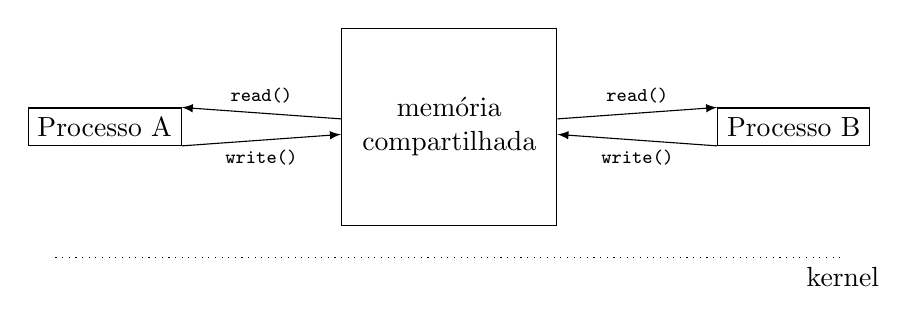
\begin{tikzpicture}
\def\shift{2.5cm}
\def\yshift{\shift/1.5}
\tikzset{base/.style={draw},
mem/.style={base,minimum width=\shift,minimum height=\shift,align=center},
proc/.style={base},
every path/.style={>=latex,draw},syscal/.style={font=\scriptsize\tt}}
\node[mem,text width=\shift] at (0,0) (MEM) {memória\\ compartilhada};
\node[proc] at (-1.75*\shift,0) (PA) {Processo A};
\node[proc] at (1.75*\shift,0) (PB) {Processo B};
\path[->] (PA.south east) -- node[syscal,below]{write()} (MEM);
\path[->] (MEM) -- node[syscal,above]{read()} (PA.north east);
\path[->] (MEM) -- node[syscal,above]{read()} (PB.north west);
\path[->] (PB.south west) -- node[syscal,below]{write()} (MEM);
\draw[dotted] (-2*\shift,-\yshift) -- (2*\shift,-\yshift) node[below] {kernel};
\end{tikzpicture}
\end{center}

